\documentclass[titlepage]{jsarticle}
\usepackage[dvipdfmx]{graphicx}
\usepackage{url}
\usepackage{amsmath}
\usepackage{siunitx}
\usepackage{comment}
\usepackage[version=3]{mhchem}
\usepackage{otf}
\title{14.フォトニクス実験}
\author{学生番号03180523 渡辺耕坪}
\date{\today}
\begin{document}
\maketitle

\begin{comment}
\begin{figure}[htbp]
 \begin{minipage}{0.5\hsize}
  \begin{center}
   \includegraphics[width=80mm]{}
  \end{center}
  \caption{}
  \label{}
 \end{minipage}
 \begin{minipage}{0.5\hsize}
  \begin{center}
   \includegraphics[width=80mm]{}
  \end{center}
  \caption{}
  \label{}
 \end{minipage}
\end{figure}
\end{comment}

\begin{comment}
\begin{figure}[htbp]
 \begin{minipage}{0.5\hsize}
  \begin{center}
   \includegraphics[width=80mm]{}
  \end{center}
  \caption{}
  \label{} \end{minipage}
\end{figure}
\end{comment}
\section{Abstract}
フォトニクス実験では半導体レーザー、超短パルスファイバレーザ、空間光学の三つに関する実験を行った。このうち超短パルスファイバレーザに関しては実験の原理、実験結果、詳細な考察を提出し、空間光学、半導体レーザーに関しては簡略な実験結果といくつかの考察のみをレポートとして提出する。
\section{Introduction}
\subsection{超短パルスファイバレーザ}
光の広い周波数帯域を利用して、時間領域で極めて狭い間のみに光パワーが集中しているパルスを発生させることができる。今回の実験ではファイバレーザを用いてパルスを発生させる。また、パルスを用いて超短パルスの時間幅を、応答時間が長いフォトディテクタによって観測する自己相関法による解析を行い、スペクトラムアナライザによって得られた結果と比較する。
\subsection{実験の原理}
\subsubsection{超短パルスファイバレーザ}

\subsection{実験装置}
オシロスコープ\\
スペクトラムアナライザ\\
半導体レーザドライバ\\
温度コントローラ\\
波形発生装置\\
直流電源\\
パソコン\\
\subsection{実験方法}
\subsubsection{半導体レーザー}
1.半導体レーザの静特性\\
温度の条件を変化させつつ、最大逆方向電流5[mA]から最大順方向電流+40[mA]までの範囲でコンピュータプログラムによる自動制御を使用し、以下の5点のレーザ静特性について計測を行う。
\begin{itemize}
    \item 電圧ー注入電流(V-I)特性
    \item 微分コンダクタンスー注入電流($\frac{dI}{dV}-I$)特性
    \item 光出力ー注入電流(P-I)特性
    \item 外部微分効率ー注入電流(P-I)特性
    \item 内臓PD出力ー注入電流(PDによるV-I)特性
\end{itemize}
温度の変化は10[\si{\degreeCelsius}],20[\si{\degreeCelsius}],40[\si{\degreeCelsius}],60[\si{\degreeCelsius}]で行う。低温条件下での結露を最小限に抑えるために20[\si{\degreeCelsius}]から始め高温側の条件下での測定を終えた後10[\si{\degreeCelsius}]の条件を測定する。\\
また、この結果よりレーザ動作を行うようになる閾値注入電流を求めることができる。
2.半導体レーザの偏光特性\\
温度を室温に固定し、レーザをポラライザに通してLDへと入力する。レーザ発振動作領域とLED動作領域のそれぞれで、ポラライザの角度に対する光検出強度の依存性を計測する。\\
次に、レーザー発振領域において、TE偏光強度ー注入電流特性、TM偏光強度ー注入電流特性を測定し、TE偏光とTM偏光の強度比の注入電流依存性を求める。\\
3.光スペクトル
図\ref{fig:exp3}のような実験系を組み、スペクトルアナライザを以下のように設定し、レーザーのスペクトルを計測する。
\begin{itemize}
    \item Amplitude-Sensitivity;-70[\si{dB}]
    \item Wavelength-Span;20[\si{nm}]
    \item Bandwidth-ResBW;最小値
\end{itemize}
温度を20[\si{\degreeCelsius}]に固定し、注入電流を閾値電流以下と閾値電流以上の両方の領域で選び、注入電流をパラメタとして発光スペクトルを観測する。\\
次に、光出力を一定値にして(PD出力が一定になるようにして)温度を10[\si{\degreeCelsius}],20[\si{\degreeCelsius}],30[\si{\degreeCelsius}],40[\si{\degreeCelsius}],50[\si{\degreeCelsius}],60[\si{\degreeCelsius}]で行う。低温条件下での結露を最小限に抑えるために20[\si{\degreeCelsius}]から始め高温側の条件下での測定を終えた後10[\si{\degreeCelsius}]の条件を測定する。\\
加えて、発振波長ー注入電流特性と細かい発振波長ー温度特性を測定する。\\
発振波長ー注入電流特性は大きい注入電流から小さい注入電流へ向けて1[\si{mA}]程度の刻み幅で測定する。\\
発振波長ー温度特性は20[\si{\degreeCelsius}]から30[\si{\degreeCelsius}]まで温度を上げていく過程で測定してから30[\si{\degreeCelsius}]から20[\si{\degreeCelsius}]まで温度を下げていく過程で測定する。


%\subsubsection{空間光学}



\subsubsection{超短パルスファイバレーザ}
1.ファイバレーザのモード同期\\
    ファイバレーザ発生システム内の個々の機器の電源を投入し、レーザ注入電流を700mAに設定する。オシロスコープで波形を見ながらシステム内の三枚の波長版を回転させ、パルスが発生するように調整する。\\
2.単一パルスを発生させる\\
    発生させたパルスはオシロスコープの表示では単一のパルスに見えるが、スペクトラムアナライザで周波数成分を見ると単一のパルスではないことが分かる。そこで、で注入電流を下げていき、スペクトル分布がどのように変化していくかを記録す
    る。\\
3.自己相関波形の解析\\
    図\ref{fig;palse_laser}の実験系を用いて単一パルスを二つに分け、経路によって時間差がついた二つの波形の重ね合わせを、二つのフォトディテクターによって観測する実験である。本来は発生させた単一パルスを用いてこの実験を行う予定だったが、実験系の不調により、あらかじめ以上の実験系を用いて行われた実験データを用いて以下の解析を行う。\\
    1.PD\\
        \ce{InGaAs}を材料とするフォトディテクターで、受光した光波の振幅の2乗に比例した電流を発生させる。\\
    2.TPA-PD\\
        \ce{GaAsP}を材料とするフォトディテクターで、受講した硬派の振幅の4乗に比例した電流を発生させる。\\
    それぞれ観測した電流を用いて離散フーリエ変換によって光スペクトルを得ることができる。これによって得られた光スペクトルを別途、スペクトラムアナライザによって得た結果と比較する。\\



\section{Results}
\subsection{半導体レーザー}
\begin{figure}[htbp]
 \begin{minipage}{0.5\hsize}
  \begin{center}
   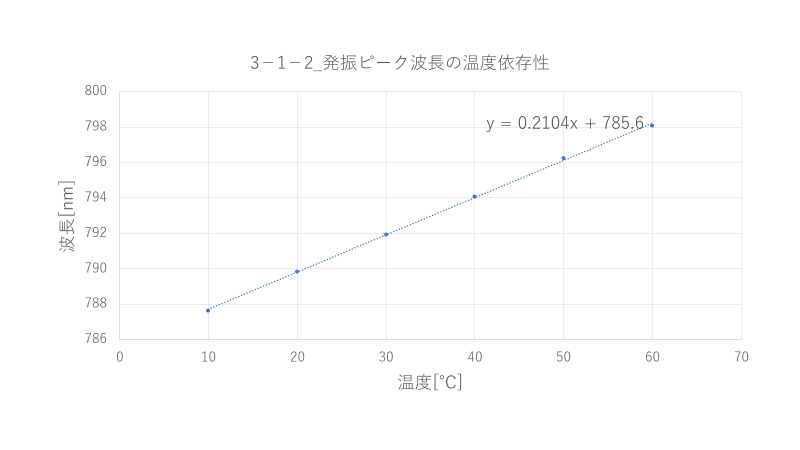
\includegraphics[width=80mm]{3_1_2.png}
  \end{center}
  \caption{10[\si{\degreeCelsius}]刻みで測定した場合の発振波長の温度依存性。0.21[\si{nm/\degreeCelsius}]の傾きを有していることが分かる}
  \label{fig:3-1-2} \end{minipage}
\end{figure}

\begin{figure}[htbp]
 \begin{minipage}{0.5\hsize}
  \begin{center}
   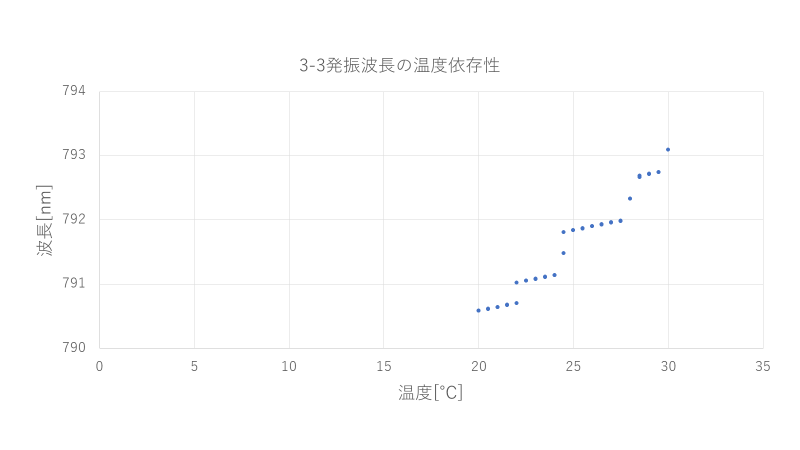
\includegraphics[width=80mm]{3-3.png}
  \end{center}
  \caption{0.5[\si{\degreeCelsius}]刻みで測定した場合の発振波長の温度依存性。モードホッピングが生じていることと、3-1-2で観測されたものより緩やかな温度依存性が生じていることが分かる。なお、文献\cite{laser_base},\cite{text}に記されているようなヒステリシスは観測できなかった。}
  \label{fig:3-3}
 \end{minipage}
 \begin{minipage}{0.5\hsize}
  \begin{center}
   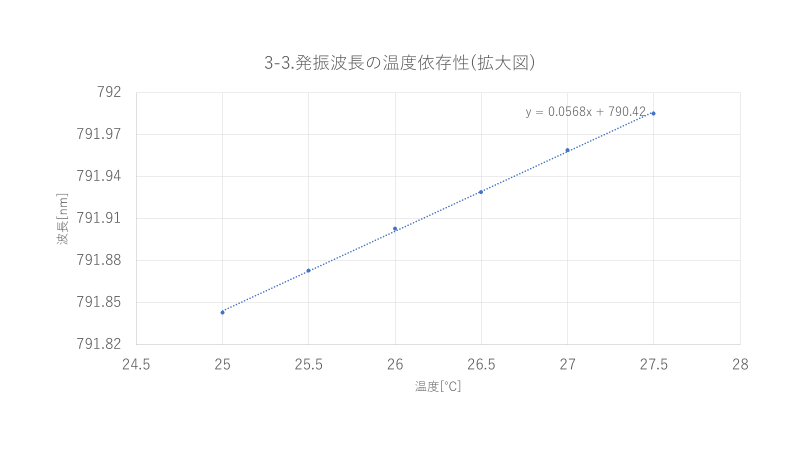
\includegraphics[width=80mm]{3-3-large.png}
  \end{center}
  \caption{左図の拡大版。緩やかな温度依存性は0.056[\si{nm/\degreeCelsius}]程度の傾きを有していることが分かる。}
  \label{fig:3-3-expand}
 \end{minipage}
\end{figure}

\subsection{空間光学}

\subsection{超短パルスファイバレーザー}
\begin{figure}[htbp]
 \begin{minipage}{0.5\hsize}
  \begin{center}
   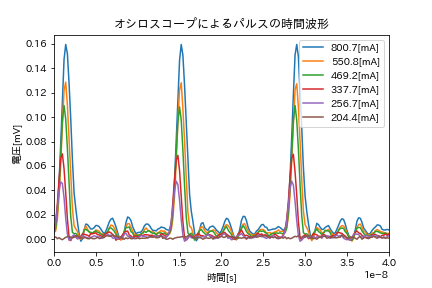
\includegraphics[width=80mm]{palse_osiro.png}
  \end{center}
  \caption{パルスをオシロスコープによって観測した結果。注入電流が大きい場合はパルスの大きさが大きいがパルス幅が広くなっている。また、注入電流が小さすぎるとノイズのみが出力されている。}
  \label{} \end{minipage}
\end{figure}
\begin{figure}[htbp]
 \begin{minipage}{0.5\hsize}
  \begin{center}
   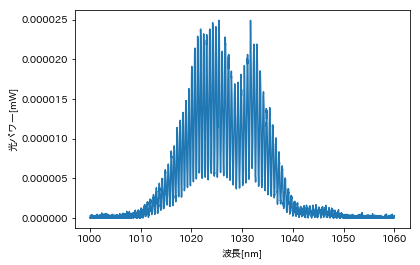
\includegraphics[width=80mm]{800_7[mA].png}
  \end{center}
  \caption{800.7[mA]の注入電流によるスペクトル。}
  \label{fig:800_7}
 \end{minipage}
 \begin{minipage}{0.5\hsize}
  \begin{center}
   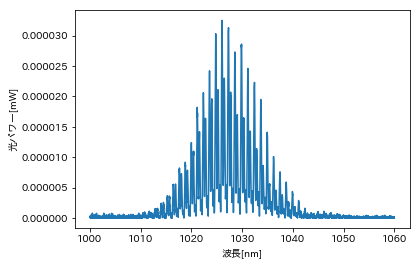
\includegraphics[width=80mm]{550_8[mA].png}
  \end{center}
  \caption{550.8[mA]の注入電流によるスペクトル。}
  \label{fig:550_8}
 \end{minipage}
\end{figure}
\begin{figure}[htbp]
 \begin{minipage}{0.5\hsize}
  \begin{center}
   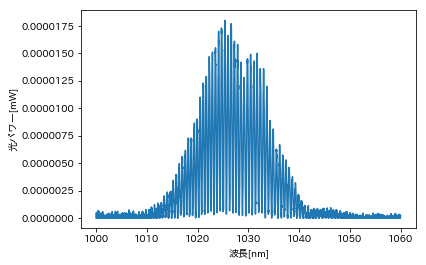
\includegraphics[width=80mm]{469_2[mA].png}
  \end{center}
  \caption{800.7[mA]の注入電流によるスペクトル。}
  \label{fig:469_2}
 \end{minipage}
 \begin{minipage}{0.5\hsize}
  \begin{center}
   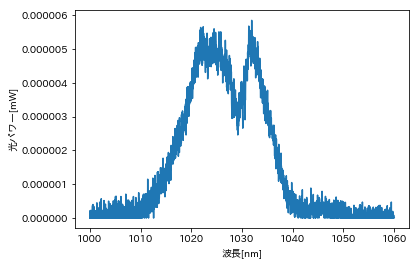
\includegraphics[width=80mm]{337_7[mA].png}
  \end{center}
  \caption{337.7[mA]の注入電流によるスペクトル。スペクトルの振動が消失している。}
  \label{fig:337_7}
 \end{minipage}
\end{figure}
\begin{figure}[htbp]
 \begin{minipage}{0.5\hsize}
  \begin{center}
   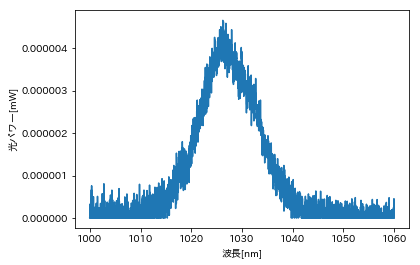
\includegraphics[width=80mm]{256_7[mA].png}
  \end{center}
  \caption{256.7[mA]の注入電流によるスペクトル。ガウシアンに近いスペクトル分布が得られた。}
  \label{fig:256_7}
 \end{minipage}
 \begin{minipage}{0.5\hsize}
  \begin{center}
   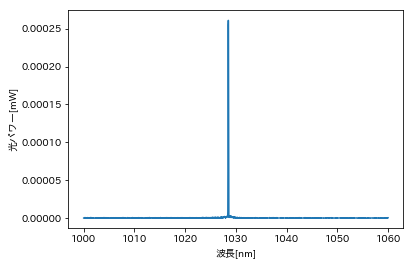
\includegraphics[width=80mm]{204_4[mA].png}
  \end{center}
  \caption{204.4[mA]の注入電流によるスペクトル。ほとんど周波数に依存する成分を得られなかったので$\delta$関数的なスペクトル分布になっている。}
  \label{fig:204_4}
 \end{minipage}
\end{figure}

\begin{figure}[htbp]
 \begin{minipage}{0.5\hsize}
  \begin{center}
   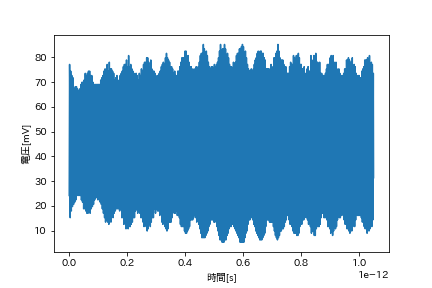
\includegraphics[width=80mm]{not_sync_208mAPD.png}
  \end{center}
  \caption{注入電流が208[mA]であり、低注入電流なので非同期モード状態のPD出力。}
  \label{fig:notsync}
 \end{minipage}
 \begin{minipage}{0.5\hsize}
  \begin{center}
   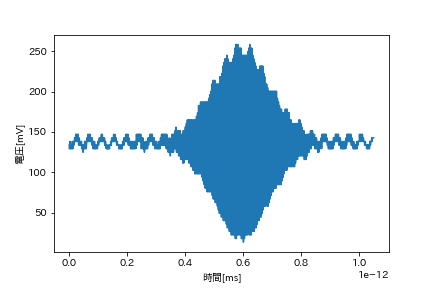
\includegraphics[width=80mm]{askT.png}
  \end{center}
  \caption{注入電流が406[mA]であり、高注入電流なので同期モード状態のPD出力。}
  \label{fig:sync}
 \end{minipage}
\end{figure}

\begin{figure}[htbp]
 \begin{minipage}{0.5\hsize}
  \begin{center}
   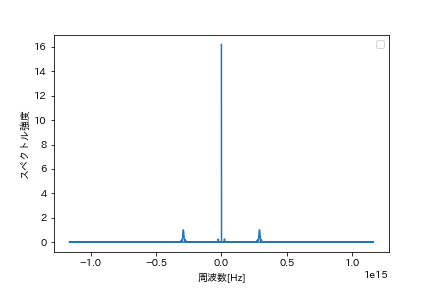
\includegraphics[width=80mm]{spectrum_all.png}
  \end{center}
  \caption{図\ref{fig:sync}の波形を離散フーリエ変換した結果。同じスペクトル分布が周波数0を軸として左右対称に表れており、一つの周波数をピークにして分布していることが分かる。}
  \label{fig:PD_spectrum}
 \end{minipage}
 \begin{minipage}{0.5\hsize}
  \begin{center}
   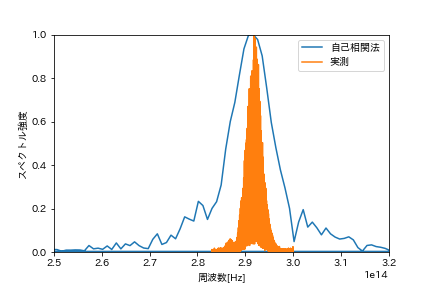
\includegraphics[width=80mm]{spectrum.png}
  \end{center}
  \caption{低周波領域を無視してスペクトル分布が生じている部分のみを切り取り、実測のスペクトル分布と比較した図。実測のスペクトル分布よりも自己相関法による解析のほうがスペクトル幅が広がってしまっていることが分かる。}
  \label{fig:spectrum_relation}
 \end{minipage}
\end{figure}

\begin{figure}[htbp]
 \begin{minipage}{0.5\hsize}
  \begin{center}
   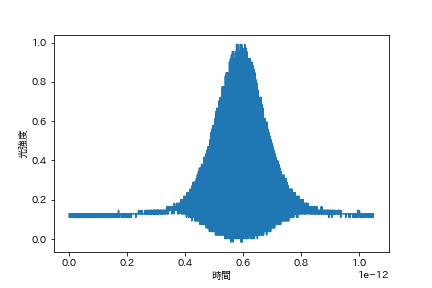
\includegraphics[width=80mm]{TPAPD.png}
  \end{center}
  \caption{TPA-PDでの時間領域での計測結果。}
  \label{fig:TPAPD_osiro}
 \end{minipage}
 \begin{minipage}{0.5\hsize}
  \begin{center}
   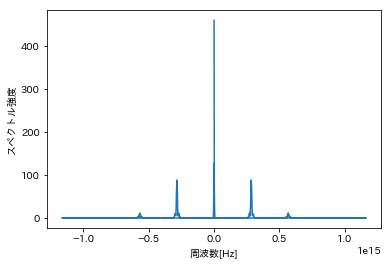
\includegraphics[width=80mm]{TPAPD_spectrum.png}
  \end{center}
  \caption{\ref{fig:TPAPD_osiro}の波形を離散フーリエ変換した結果。ある周波数とその二倍の周波数にを中心としてスペクトル分布が生じていることが分かる。}
  \label{fig:TPAPDspectrum}
 \end{minipage}
\end{figure}

\begin{figure}[htbp]
 \begin{minipage}{0.5\hsize}
  \begin{center}
   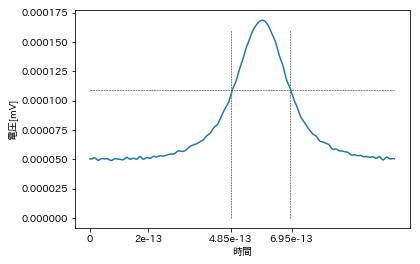
\includegraphics[width=90mm]{FWHM.png}
  \end{center}
  \caption{時間領域でのFWHMの見積もり。FWHMは2.1e-13[s]となった。}
  \label{FWHM} \end{minipage}
\end{figure}
\clearpage
\section{Discussion}
\subsection{半導体レーザー}
五つある発表課題のうち発表課題5について考察を行う。\\
\subsubsection{二種類の温度依存性について}
図\ref{fig:3-1-2},\ref{fig:3-3-expand}から読み取れる通り、3-1-2では0.21[\si{nm/\degreeCelsius}]の傾きの温度依存性が観測され、3-3では0.056[\si{nm/\degreeCelsius}]程度の傾きの温度依存性が観測された。まず、緩やかな温度依存性については、屈折率の温度依存性によるものと考えられ、比較的大きな傾きの温度依存性は光利得曲線の温度上昇に伴う長波長へのシフトであると考えれる。
\subsubsection{屈折率の温度依存性}
Varshniの経験式\cite{varshini}の経験式に基づくと、温度上昇に伴ってバンドギャップは小さくなる。(温度とバンドギャップの関係は\cite{bandgap}などで議論されているように一般的には複雑である。十分高温下の条件では、定性的には、温度上昇に伴って最近接原子同士の波動関数の重なりが増え、許容帯が広くなり、バンドギャップが狭まると考えられている\cite{QandA})\\
バンドギャップが縮むと、物質の光の吸収
クラマース-クローニッヒの関係によって複素屈折率の実部も同時に上昇し、屈折率が上昇する。\\
屈折率が上昇すると、定在波が立つ条件
\begin{align}
    \label{lambda}
    \frac{\lambda}{2n_{eff}}m=L(m=0,1,2…,Lは干渉計の長さ)
\end{align}
式\ref{lambda}の$n_{eff}$が上昇するので、mを固定した場合の$\lambda$も上昇していく。
\subsubsection{比較的大きな温度依存性}
単に式\ref{lambda}を満たし、立っている定在波の利得は、波長依存性がないが、これに光利得曲線の効果が加わると、上に凸な光利得曲線が包絡線となり、ピークの発振波長が作られる。光利得曲線は\cite{}で議論されているような温度依存性を持つ。光利得曲線が温度上昇に伴って高波長へとシフトしていくことでピークの発振波長も高温側へとシフトしていくと考えられる。
\subsubsection{組成式の見積もり}
\cite{datasheet}内の
\begin{align}
    \label{E_g}
    E_g=E(0)-\frac{5.41\times10^{-4}\times T^2}{T+204}\\
    E(0)=1.519+1.155x+0.37x^2
    \label{E_0}
\end{align}
に対して、xを目的変数、Tを説明変数として最小二乗法によってxをフィッティングする(図\ref{fig:stimulate_x})。その結果、見積もられたxの値は0.12となった。
\begin{figure}[htbp]
 \begin{minipage}{0.5\hsize}
  \begin{center}
   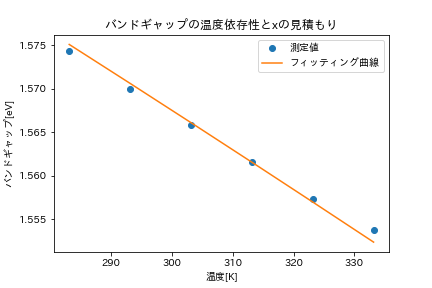
\includegraphics[width=80mm]{stimulate_x.png}
  \end{center}
  \caption{scipyのcurve\_fitによってフィッティングを行った。}
  \label{fig:stimulate_x} \end{minipage}
\end{figure}
\subsubsection{高電流下での発熱による温度上昇の見積もり}
実験3-1-1の注入電流を20[mA]としたときの発振波長からバンドギャップを求めると、発振波長は787.62[\si{nm}]である。発振波長[\si{nm}]からバンドギャップ$E_g[\si{eV}]$は、$E_g=\frac{1440}{\lambda}$に波長を代入すれば求められることが知られているので、これにより計算を行うと、バンドギャップは
1.56\si{[eV]}である。式
\ref{E_g},\ref{E_0}にこのバンドギャップの値と求められたxの値を代入すると、Tを求められる。その結果は305[K]となり、ペルチェ素子による温度制御が20[\si{\degreeCelsius}]であるのに対して温度は約32[\si{\degreeCelsius}]まで上昇していることが分かる。\\
このようにして推定された温度の妥当性を、微分効率の温度依存性から評価したい。まず、レーザ発振領域で注入電流が小さい状態では温度変化が十分小さいと考えられる。低注入電流条件下での20[\si{\degreeCelsius}]と40[\si{\degreeCelsius}]での微分効率を計算し、30[\si{\degreeCelsius}]程度での微分効率を見積もる。20[\si{\degreeCelsius}]かつ高注入電流条件下での微分効率も別途計算し、前述のように見積もられた微分効率と比較し、妥当性を評価する。\\
しかし、発振の閾値電流が15[\si{mA}]程度であり、高注入電流条件は最大でも20[\si{mA}]の条件しか測定していなかったため、注入電流の差が反映されているとは考えづらい実験データになってしまった。各条件の微分効率の比較は図\ref{fig:stimulate_T}のようになった。結果的には、微分効率の温度依存性は極めて弱いため、三条件の中で見られる微分効率の変動はノイズのレベルであり、有意な差ではないと考えられる。
\begin{figure}[htbp]
 \begin{minipage}{0.5\hsize}
  \begin{center}
   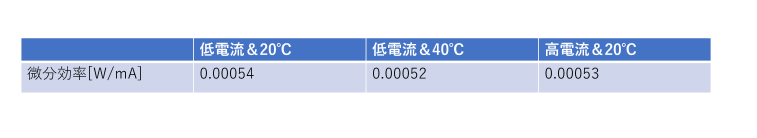
\includegraphics[width=160mm]{stimulate_T.png}
  \end{center}
  \caption{3条件の微分効率の比較。高電流&20[\si{\degreeCelsius}]の条件は見積もりによると低電流&30[\si{\degreeCelsius}]の微分効率と一致するはずであり、そのような結果となっているが、微分効率の温度依存性はこの温度幅では極めて低いため、有意なものではないと考えられる}
  \label{fig:stimulate_T} \end{minipage}
\end{figure}

\subsection{超短パルスレーザー}
検討課題1~4と7について考察を行う。
1.
\begin{equation}
    S(t)=\frac{1}{2}[\varepsilon(t)e^{j\omega_0 t}+c.c](c.cは直前項の複素共役を表す)
    \label{eq1_1}
\end{equation}
\begin{equation}
    S(\omega)=\frac{1}{2}[E(\omega-\omega_0)+E^{*}(-\omega-\omega_0)]
    \label{eq1_2}
\end{equation}
式\ref{eq1_1}をフーリエ変換し$S(\omega)とE(\omega)$が式\ref{eq1_2}の関係となっていることを示す。\\
2.レーザーからダブルパルスが出力されているときスペクトルが振動する理由。また、振動周期から推定されるダブルパルスの時間幅について。\\
3.レーザの平均パワーが10[W]程度であると仮定し、繰り返し周波数
とパルス幅を用いてピークパワーを推定する。\\
4.計測された光パルスの時間幅は光の何周期分か推定する。また、スペクトル幅と中心周波数の比と、両者の関係について。\\
7.ガウシアンパルスのスペクトル位相が$\Phi(\omega)=-\frac{1}{2}\Phi_2\omega^2$であるときの時間波形の計算。\\


\section{Summary}


\begin{thebibliography}{9}
  \bibitem{laser_base}栖原敏明、半導体レーザの基礎、共立出版(1998)
  \bibitem{text}電気電子情報実験・演習第二 2018年度東京大学工学部電気系学科
  \bibitem{datasheet}\ce{AlGaAs}のデータシート\url{http://www.ioffe.ru/SVA/NSM/Semicond/AlGaAs/bandstr.html}
  \bibitem{varshini} Temperature dependence of the energy bandgap \url{https://ecee.colorado.edu/~bart/book/eband5.htm}
  \bibitem{bandgap} 是常 隆 新学術領域研究「コンピューティクスによる物質デザイン」平成25年度研究会 半導体バンドギャップの温度依存性  \url{http://computics-material.jp/files/symposium/20140310-11/document/29_koretsune_document.pdf}
  \bibitem{QandA} 佐藤勝昭 科学技術振興機構 \url{http://home.sato-gallery.com/research/crystal_letters_nandemoQA(14).pdf}
\end{thebibliography}
\end{document}

